\documentclass[a4,10truept]{jsarticle}
\usepackage[top=24truemm,bottom=24truemm,left=22truemm,right=22truemm]{geometry}
\usepackage{graphicx}
\usepackage{bm}
\usepackage{wrapfig}
\usepackage{abstract}
\usepackage{cite}
\renewcommand{\baselinestretch}{1}
\renewcommand{\abstractname}{}
\renewcommand{\absnamepos}{empty}
\pagestyle{empty}
\usepackage{titlesec}
\titleformat*{\section}{\fontsize{12.5truept}{0truept} \bf \gt}
\makeatletter
 \DeclareRobustCommand\cite{\unskip
\@ifnextchar[{\@tempswatrue\@citex}{\@tempswafalse\@citex[]}}
% \def\@cite#1#2{$^{\hbox{\scriptsize{#1\if@tempswa , #2\fi})}}$}
\def\@cite#1#2{$^{\hbox{\scriptsize{#1\if@tempswa , #2\fi}}}$}
 \def\@biblabel#1{#1)}
\makeatother


%https://qiita.com/Toru3/items/7ea1342da1e31f0c28c3
\usepackage{fancyhdr}
\usepackage{lastpage}
\fancypagestyle{mypagestyle}{%
\lhead{\thepage/\pageref{LastPage}}%ヘッダ左
\rhead{研究論文の要旨1 (出版論文の要旨) 平松信義}%ヘッダ右
\cfoot{}%\thepage/\pageref{LastPage}}%フッタ中央に"今のページ数/総ページ数"を設定
\renewcommand{\headrulewidth}{0.0pt}%ヘッダの線を消す
}
\pagestyle{mypagestyle}
\usepackage{comment}

\title{研究論文の要旨1 (出版論文\thanks{Nobuyoshi Hiramatsu, Fumiya Kusa, Kotaro Imasaka, Ikki Morichika, Akinobu Takegami, and Satoshi Ashihara, Propagation length of mid-infrared surface plasmon polaritons on gold: Impact of morphology change by thermal annealing, Journal of Applied Physics {\bf 120}, 173103 (2016)
} の要旨)\\
金表面における中赤外プラズモンポラリトンの伝搬長測定}

\author{平松信義$\!^{1,2)}$, 草史野$\!^{1,3)}$, 竹上明伸$\!^{1,3)}$, 今坂光太郎$\!^{1)}$, 森近一貴$\!^{1)}$, 芦原聡$\!^{1,\mathrm{a})}$\\ 東京大学生産技術研究所$\!^{1)}$, 東京大学物理工学科$\!^{2)}$, 東京農工大学物理システム工学専攻~$\!^{3)}$}
\date{}
\begin{document}
\maketitle
\thispagestyle{mypagestyle}

%\vspace{-0.3em}
\begin{abstract}
{\fontsize{10pt}{0pt} 金/空気界面を伝搬するプラズモンポラリトン(SPP)の伝搬長を中赤外域で測定した。波長$10.6\:\mathrm{\mu m}$でSPPは10mm以上伝搬し、多結晶の金の誘電率から計算される伝搬長とよく一致することを示した。またSPPの導波デバイスをアニールすることで結晶粒が大きく、表面荒さは小さくなり、SPPの伝搬長が大きくなることを示した。}
%{\fontsize{10pt}{0pt} \rm We studied propagation length of surface plasmon polaritons (SPPs) at gold/air interface in the mid-infrared range. We showed that SPPs propagate for a distance of about or above $10\:\mathrm{mm}$ at a wavelength of $10.6\:\mathrm{\mu m}$, in good agreement with the value predicted from dielectric constant of polycrystalline gold. We also demonstrated that a simple treatment of thermal annealing led to noticeable elongation of SPP propagation length, accompanied by increased grain size and decreased surface roughness.}
\end{abstract}

%\vspace{-0.7em}
\section{赤外プラズモニクス}
\vspace{-0.5em}
\mc 赤外プラズモニクスは,  表面増強分光やバイオセンサ, 輻射制御, プラズモニック回路などへの応用の可能性から, 近年注目を集めている. 特に赤外域のプラズモニック材料として金は, 化学的に安定で, オームロスが小さいため, 広く用いられている. 
ここで, これらの性能は表面プラズモン励起により得られる電場増強度と関連しており, 一般的にプラズモンポラリトン(SPP)の伝搬長で特徴づけられる. 
これまで赤外域において金表面を伝搬するSPPの伝搬長はいくつか報告されてきたが\cite{McMullen,Schlesinger1,Schlesinger2}, 試料のモルフォロジーの観点からの考察が欠けており, お互いに定量的な一致を見ていない. 本研究の目的は, 中赤外域で金-空気界面を伝搬するSPPの伝搬長と金のモルフォロジーをあわせて評価することで, 伝搬長とモルフォロジーとの相関を示すことにある. 

\vspace{-0.2em}
\section{デバイスおよび実験方法}
\vspace{-0.5em}
%\setlength{\intextsep}{0pt}
\setlength{\columnsep}{1em}%
\begin{wrapfigure}{R}[0mm]{0.45\hsize}
  \centering
  \raisebox{0pt}[\dimexpr\height-\baselineskip\relax]{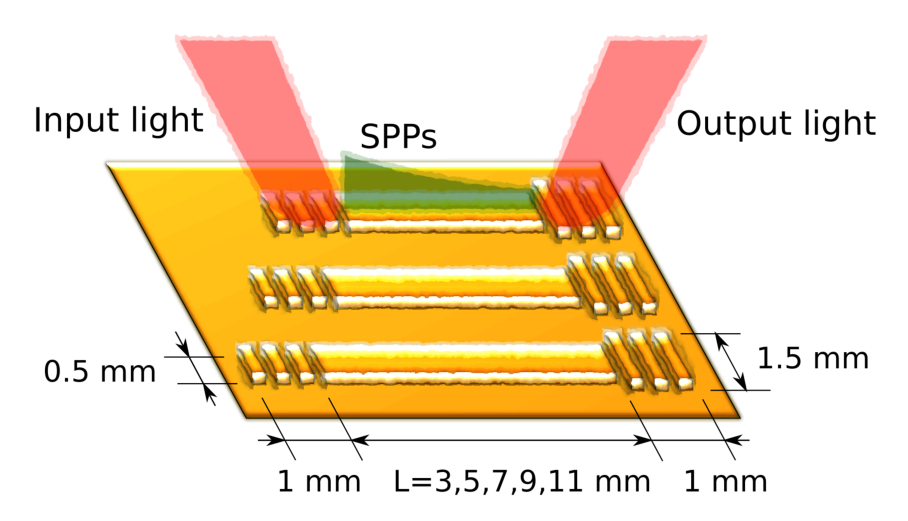
\includegraphics[width=\hsize]{schematic.eps}}
    \caption{SPP導波デバイスの模式図}
     \label{fig:schematic}
\end{wrapfigure}
SPPの伝搬長を測定するために, 図1に示すような一対の回折格子(入力/出力カップラー)と長さの異なるSPP導波路からなるデバイスの組を作成した. SPPは, まず自由空間伝搬光により入力カップラーで励起され, 導波路表面を伝搬し, 再び出力カップラーで伝搬光と結合する. ここで入力光と出力光のパワーの比は, 伝搬光とSPPの結合効率, SPPの伝搬効率(透過率), SPPと伝搬光の再結合効率の積で与えられ, 導波路の長さに依存して減衰する指数関数に従う. したがって入射光パワーとSPP-伝搬光結合効率を一定とすると, 各デバイスについて出力光のパワーを測定することにより伝搬長(SPPのパワーが1/eに落ち込む距離)が評価できる. 

光源には$\mathrm{CO_2}\!$レーザー(波長$10.6\:\mathrm{\mu m}$)を用いた. 入力/出力カップラー(溝深さ800 nm)と導波路(厚さ800 nm)の構造は, シリカ基板に蒸着された金下地(厚さ200 nm)の上に, さらに電子線リソグラフィーと金の熱蒸着を行うことで作成した. カップラーは表面リリーフ回折格子であり, 溝深さは厳密結合波解析法による計算で最適化した. 
金のモルフォロジーを制御するために試料は$600\:\mathrm{^\circ C}$ (20分)と$700\:\mathrm{^\circ C}$ (16分)で2段階アニール処理し, そのモルフォロジーを原子間力顕微鏡(AFM)を用いて評価した.

\vspace{-0.2em}
\section{SPP伝搬長の測定とモルフォロジー観測}
\vspace{-0.5em}
\begin{wrapfigure}{r}[0mm]{0.5\hsize}
  \centering
\begin{minipage}{\hsize}
     \raisebox{0pt}[\dimexpr\height-\baselineskip\relax]{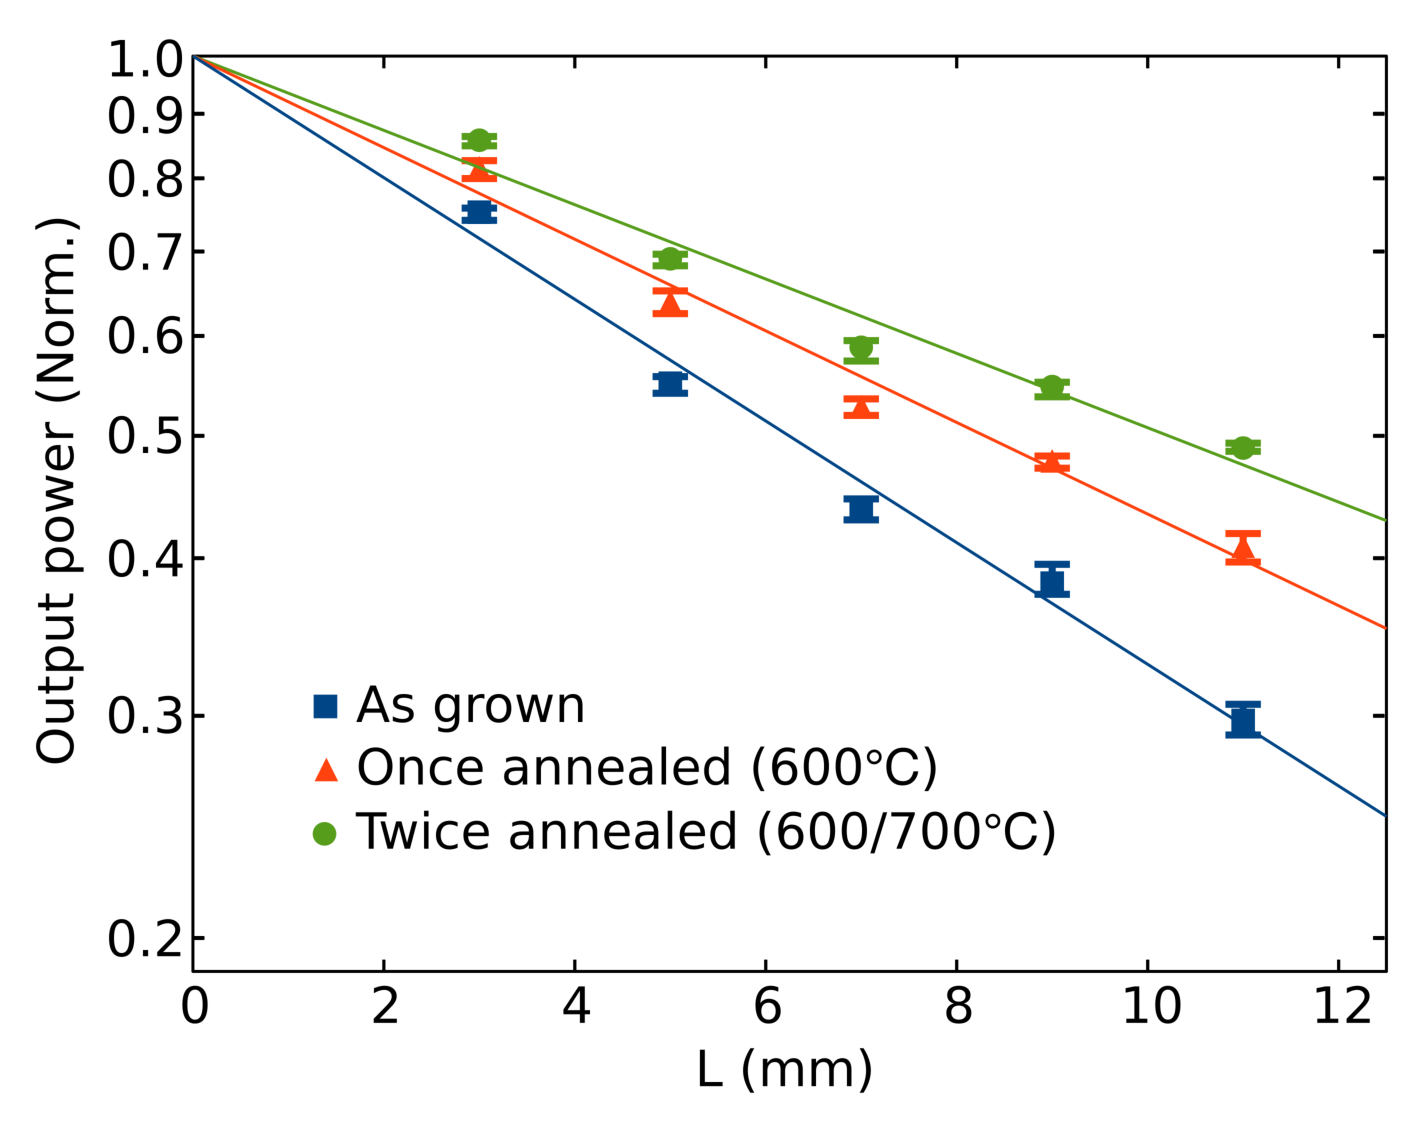
\includegraphics[width=0.9\hsize]{propagation_length.eps}}
    \caption{SPP導波デバイスの長さ$L$と規格化された出射光パワーの関係}
       \label{fig:propagation_length}
\end{minipage}\\
\begin{minipage}{\hsize}
     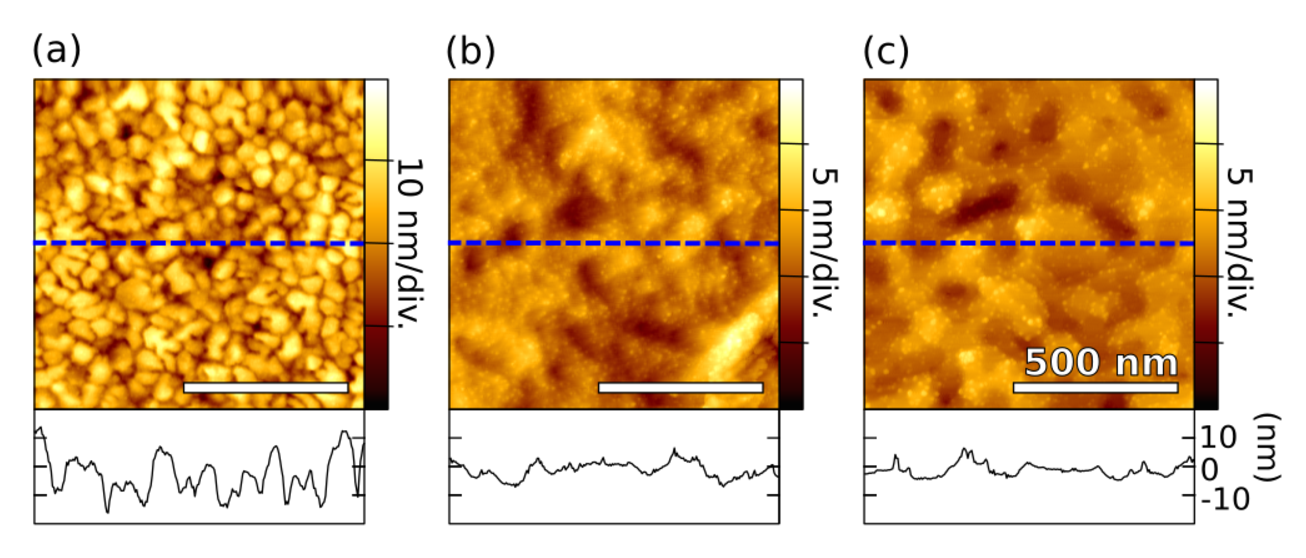
\includegraphics[width=\hsize]{morphology.eps}
        \caption{サンプルA, B, CそれぞれのAFMトポグラフィー画像と断面の高さ曲線}
    \label{fig:morphology}
\end{minipage}
\end{wrapfigure}
導波路長さ$L$の関数である出力光パワーを, アニール前の試料(A), アニールを1回施した試料(B), アニールを2回施した試料(C)それぞれについて図2にプロットした. ここで出力光パワーは, それぞれの試料で指数フィッティングされており(実線), $L=0$の値をもとに正規化されている. 伝搬長さは試料A, B, Cに対してそれぞれ$9.0\pm0.3\:\mathrm{mm}$, $12.0\pm0.4\:\mathrm{mm}$, $14.7\pm0.7\:\mathrm{mm}$であり, アニールにより伝搬長が大きくなったことがわかる. この測定結果は金多結晶の誘電率\cite{Palik}による計算$12.3\:\mathrm{mm}$とよく一致した. 

導波路表面でのAFMトポグラフィとその断面(トポグラフィ中の破線領域)を, 試料A,B,Cのそれぞれについて図3(a,b,c)に示した. 表面荒さは試料A, B, Cのそれぞれで5.7 nm, 2.8 nm, 2.2 nmであり, アニールにより表面荒さが小さくなったことがわかる. 図3(a)から試料Aについて, 多結晶に特有の結晶粒が明確に確認でき, その直径を$70\pm20\:\mathrm{nm}$と見積もった. アニール後の試料B,Cの結晶粒界はAFMトポグラフィからは不明瞭であるが, 結晶粒が大きくなったことが見て取れ, 電子後方散乱回折法による分析からも結晶粒の拡大が確認された. 

本研究でアニールによりSPP伝搬長が大きくなったメカニズムを, 結晶粒界における電子とSPPの散乱の観点から述べる. Trollmannら\cite{Trollmann}が示したように, 結晶粒が大きくなると結晶粒界での自由電子の散乱レートとそれに起因するオームロスは小さくなる. またKuttgeら\cite{Kuttge}とLeeら\cite{Lee}の報告によると, 伝搬するSPPの結晶粒界による散乱も損失に寄与する. したがって, アニールにより増大したSPPの伝搬長は, 結晶粒が大きくなり結晶粒界の密度が小さくなったことと関連付けられる. それに対して, 本研究で表面荒さの伝搬長への影響は無視できるか, 他の要因に比べ小さい. 

\vspace{-0.2em}
\section{結論}
\vspace{-0.5em}
金-空気界面を波長$10.6\:\mathrm{\mu m}$において伝搬するSPPの伝搬長が, 誘電率による計算とよく一致し, 10 mmを超えうることを実験で示した. また熱アニールの手続きによって伝搬長が大きくなると同時に, 結晶粒が大きく, 表面荒さが小さくなることを示した. SPPの伝搬長をモルフォロジーと関連付けて定量的に評価することは, プラズモニック導波路などの応用の観点のみならず, さらなるロスメカニズムの理解にも有用である. 

%\renewcommand{\refname}{}
%\bibliographystyle{unsrt}
%\bibliography{Reference}
\vspace{-0.2em}
\begin{thebibliography}{9}
\vspace{-0.5em}
\bibitem{McMullen} J. D. McMullen, Sol. Stat. Commun. {\bf 17}, 331 (1975).
\bibitem{Schlesinger1} Z. Schlesinger and A. J. Sievers, Sol. Stat. Commun. {\bf 43}, 671 (1982).
\bibitem{Schlesinger2} Z. Schlesinger and A. J. Sievers, Phys. Rev. B {\bf 26}, 6444 (1982).
\bibitem{Palik} E. D. Palik, "Handbook of Optical Constants of Solids," (Academic Press, 2002).
\bibitem{Trollmann} J. Trollmann and A. Pucci, J. Phys. Chem. C {\bf 118}, 15011 (2014).
\bibitem{Kuttge} M. Kuttge, et al., Appl. Phys. Lett. {\bf 93}, 113110 (2008).
\bibitem{Lee} H. S. Lee, et al., Opt. Exp. {\bf 20}, 8974 (2012).
%\bibitem{Mills} D. L. Mills, Phys. Rev. A {\bf 12}, 4036 (1975).
\end{thebibliography}

\end{document}